\documentclass[t]{beamer}  % [t], [c], или [b] --- вертикальное выравнивание на слайдах (верх, центр, низ)
%\documentclass[handout]{beamer} % Раздаточный материал (на слайдах всё сразу)
%\documentclass[aspectratio=169]{beamer} % Соотношение сторон

\usetheme{Boadilla} % Тема оформления
%\usetheme{Bergen}
%\usetheme{Szeged}

\usecolortheme{whale} % Цветовая схема
%\useinnertheme{circles}
%\useinnertheme{rectangles}

%\usetheme{HSE}

%%% Работа с русским языком
\usepackage{cmap}					% поиск в PDF
\usepackage{mathtext} 				% русские буквы в формулах
\usepackage[T2A]{fontenc}			% кодировка
\usepackage[utf8]{inputenc}			% кодировка исходного текста
\usepackage[english,russian]{babel}	% локализация и переносы

%% Beamer по-русски
\newtheorem{rtheorem}{Теорема}
\newtheorem{rproof}{Доказательство}
\newtheorem{rexample}{Пример}
\newtheorem{rproblem}{Задача}
\newtheorem{rsolve}{Решение}

%%% Дополнительная работа с математикой
\usepackage{amsmath,amsfonts,amssymb,amsthm,mathtools} % AMS
\usepackage{icomma} % "Умная" запятая: $0,2$ --- число, $0, 2$ --- перечисление

%% Номера формул
%\mathtoolsset{showonlyrefs=true} % Показывать номера только у тех формул, на которые есть \eqref{} в тексте.
%\usepackage{leqno} % Нумерация формул слева

%% Свои команды
\DeclareMathOperator{\sgn}{\mathop{sgn}}
\DeclareMathOperator{\card}{\mathop{card}} % Мощность множества
\DeclareMathOperator{\im}{\mathop{Im}} % Образ отображения
\DeclareMathOperator{\divergence}{\mathop{div}} % Дивергенция
\DeclareMathOperator{\rot}{\mathop{rot}} % Ротор

%% Перенос знаков в формулах (по Львовскому)
\newcommand*{\hm}[1]{#1\nobreak\discretionary{}
{\hbox{$\mathsurround=0pt #1$}}{}}

%%% Работа с картинками
\usepackage{graphicx}  % Для вставки рисунков
\graphicspath{{images/}{images2/}}  % папки с картинками
\setlength\fboxsep{3pt} % Отступ рамки \fbox{} от рисунка
\setlength\fboxrule{1pt} % Толщина линий рамки \fbox{}
\usepackage{wrapfig} % Обтекание рисунков текстом

%%% Работа с таблицами
\usepackage{array,tabularx,tabulary,booktabs} % Дополнительная работа с таблицами
\usepackage{longtable}  % Длинные таблицы
\usepackage{multirow} % Слияние строк в таблице

%%% Программирование
%\usepackage{etoolbox} % логические операторы

%%% Другие пакеты
\usepackage{lastpage} % Узнать, сколько всего страниц в документе.
\usepackage{soul} % Модификаторы начертания
\usepackage{csquotes} % Еще инструменты для ссылок
%\usepackage[style=authoryear,maxcitenames=2,backend=biber,sorting=nty]{biblatex}
\usepackage{multicol} % Несколько колонок

%%% Картинки
\usepackage{tikz} % Работа с графикой
\usepackage{pgfplots}
\usepackage{pgfplotstable}

\usepackage{xcolor}

\title{Праздничный ужин}
\subtitle{}
\author{Константин Кравцов}%
%\institute{Ужин с итальянскими наклонностями}
\date{5 июля 2020}

\begin{document}


\begin{frame}
	\maketitle
\end{frame}


\begin{frame}[c]\label{ToC}
%	\tableofcontents
	
	\begin{block}{\begin{center}Содержание\end{center}}
	\begin{center}
		\hyperlink{main}{\beamerbutton{\nameref{main}}} \\
		\hyperlink{cakes}{\beamerbutton{\nameref{cakes}}} \\
		\hyperlink{drinks}{\beamerbutton{\nameref{drinks}}} \\
	\end{center}
	\end{block}
	
\end{frame}


%\section{Главные блюда}\label{main1}
%\begin{frame}
%	\frametitle{\insertsection}
%	\framesubtitle{\href{https://bonfesto.by/recipes/filter/category-is-prazdnichnoe-menyu/apply/}{Ссылка на основной источник}}
%	\begin{itemize}
%	\begin{multicols}{2}
%		\item<1-1> Паста с базиликом и моцареллой
%		\item<2-2> Ньокки в томатном соусе
%		\item<3-3> Лазанья с фаршем
%		\only<1-1>{\item 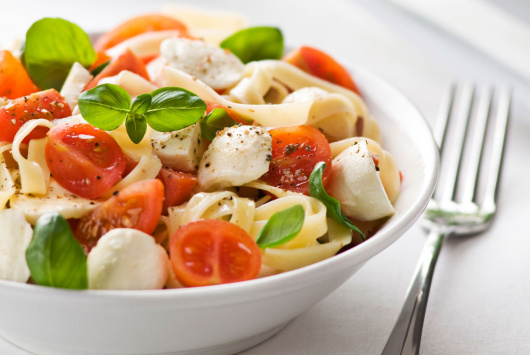
\includegraphics[scale=0.25]{Pastamozzarella}}
%		\only<2-2>{\item 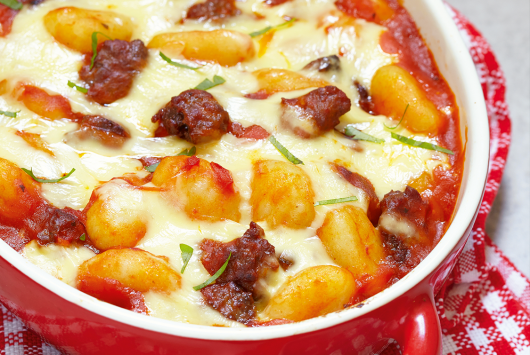
\includegraphics[scale=0.25]{Gnocchi}}
%		\only<3-3>{\item 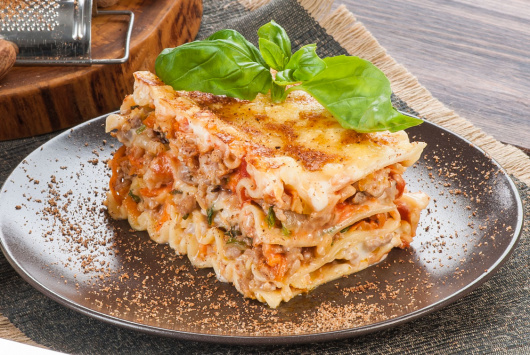
\includegraphics[scale=0.25]{Lasagna}}
%	\end{multicols}
%	\end{itemize}
%%	\begin{columns}[c]
%%		\column{1.5in}
%%		Паста с базиликом и моцареллой\\
%%		Ньокки в томатном соусе
%%		
%%		\column{1.5in}
%%		\framebox{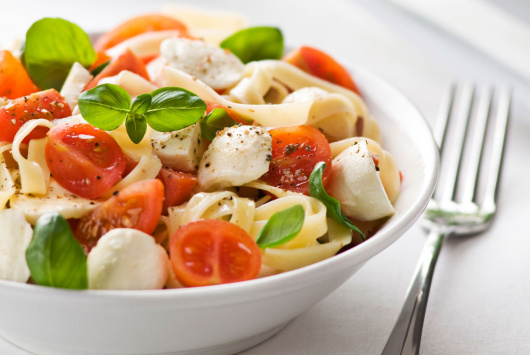
\includegraphics[scale=0.5]{Pastamozzarella}
%%	\end{columns}
%\end{frame}


\section{Главные блюда}\label{main}
\begin{frame}
	\frametitle{\insertsection}
	Все картинки для раздела \nameref{main} взяты с одного \href{https://bonfesto.by/recipes/filter/category-is-prazdnichnoe-menyu/apply/}{\textcolor{blue}{\underline{источника}}}
	\only<1-1>{
	\begin{block}{\begin{center} Паста с базиликом и моцареллой \end{center}}
		\begin{center}
		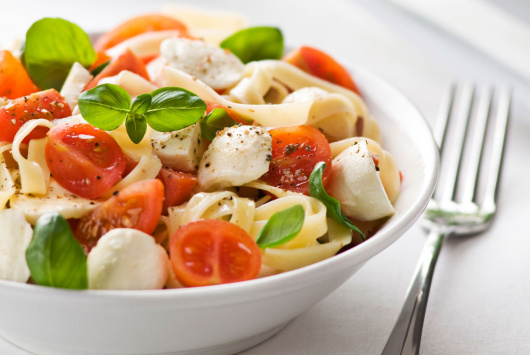
\includegraphics[scale=0.5]{Pastamozzarella}
		\end{center}
	\end{block}}
	
	\only<2-2>{
	\begin{block}{\begin{center} Ньокки в томатном соусе \end{center}}
		\begin{center}
		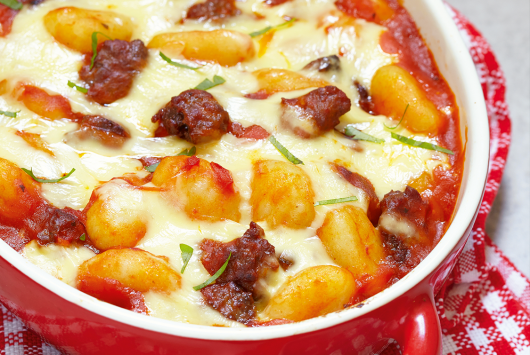
\includegraphics[scale=0.5]{Gnocchi}
		\end{center}
	\end{block}}
	
	\only<3-3>{
	\begin{block}{\begin{center} Лазанья с фаршем \end{center}}
		\begin{center}
		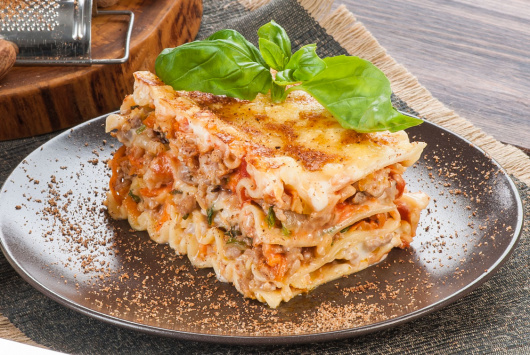
\includegraphics[scale=0.5]{Lasagna}
		\end{center}
	\end{block}}
	\uncover<3->{\hyperlink{ToC}{\beamerbutton{К содержанию}}}
\end{frame}


\section{Закуски}\label{cakes}
\begin{frame}
	\frametitle{\insertsection}
	Все картинки для раздела \nameref{cakes} взяты с одного \href{https://bonfesto.by/recipes/filter/category-is-prazdnichnoe-menyu/apply/}{\textcolor{blue}{\underline{источника}}}
	\only<1-1>{
		\begin{block}{\begin{center} Сырный пирог \end{center}}
		\begin{center}
		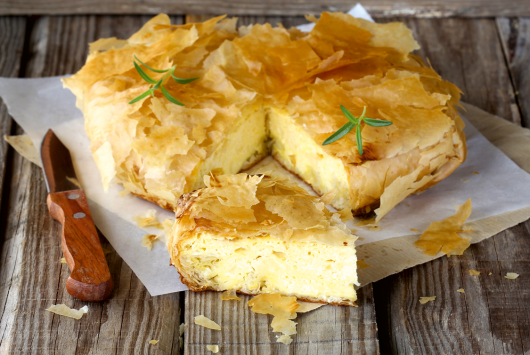
\includegraphics[scale=0.5]{Cheesecake}
		\end{center}
	\end{block}}
	\only<2-2>{
		\begin{block}{\begin{center} Стромболи с салями \end{center}}
		\begin{center}
		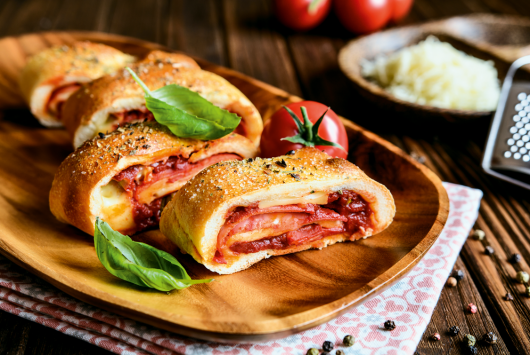
\includegraphics[scale=0.5]{Salami}
		\end{center}
	\end{block}}
	\uncover<2->{\hyperlink{ToC}{\beamerbutton{К содержанию}}}
\end{frame}


\section{Напитки}\label{drinks}
\begin{frame}
	\frametitle{\insertsection}
	\begin{center}
	\begin{itemize}
	\begin{multicols}{2}
		\item Соки
		\item Сладкие напитки
		\item Вино
		\item Минеральная вода
	\end{multicols}
	\end{itemize}
	\includegraphics[scale=0.5]{drinks}
	\end{center}
	\hyperlink{ToC}{\beamerbutton{К содержанию}}
\end{frame}


\end{document}

